\documentclass{beamer}

\mode<presentation>
{
  \usetheme{default}
  \usecolortheme{default}
  \usefonttheme{default}
  \setbeamertemplate{navigation symbols}{}
  \setbeamertemplate{caption}[numbered]
  \setbeamertemplate{footline}[page number]
  \setbeamercolor{frametitle}{fg=white}
  \setbeamercolor{footline}{fg=black}
}

\usepackage[english]{babel}
\usepackage[utf8x]{inputenc}
\usepackage{tikz}
\usepackage{listings}
\usepackage{courier}
\usepackage{array}
\usepackage{bold-extra}
\usepackage{minted}

\xdefinecolor{darkblue}{rgb}{0.1,0.1,0.7}
\xdefinecolor{darkgreen}{rgb}{0,0.5,0}
\xdefinecolor{darkgrey}{rgb}{0.35,0.35,0.35}
\xdefinecolor{darkorange}{rgb}{0.8,0.5,0}
\xdefinecolor{darkred}{rgb}{0.7,0,0}
\xdefinecolor{dianablue}{rgb}{0.18,0.24,0.31}
\definecolor{commentgreen}{rgb}{0,0.6,0}
\definecolor{stringmauve}{rgb}{0.58,0,0.82}

\lstset{ %
  backgroundcolor=\color{white},      % choose the background color
  basicstyle=\ttfamily\small,         % size of fonts used for the code
  breaklines=true,                    % automatic line breaking only at whitespace
  captionpos=b,                       % sets the caption-position to bottom
  commentstyle=\color{commentgreen},  % comment style
  escapeinside={\%*}{*)},             % if you want to add LaTeX within your code
  keywordstyle=\color{blue},          % keyword style
  stringstyle=\color{stringmauve},    % string literal style
  showstringspaces=false,
  showlines=true
}

\lstdefinelanguage{scala}{
  morekeywords={abstract,case,catch,class,def,%
    do,else,extends,false,final,finally,%
    for,if,implicit,import,match,mixin,%
    new,null,object,override,package,%
    private,protected,requires,return,sealed,%
    super,this,throw,trait,true,try,%
    type,val,var,while,with,yield},
  otherkeywords={=>,<-,<\%,<:,>:,\#,@},
  sensitive=true,
  morecomment=[l]{//},
  morecomment=[n]{/*}{*/},
  morestring=[b]",
  morestring=[b]',
  morestring=[b]"""
}

\title[2017-02-08-rootio-femtocode]{Executing code on columnar data}
\author{Jim Pivarski}
\institute{Princeton -- DIANA}
\date{February 8, 2017}

\begin{document}

\logo{\pgfputat{\pgfxy(0.11, 8)}{\pgfbox[right,base]{\tikz{\filldraw[fill=dianablue, draw=none] (0 cm, 0 cm) rectangle (50 cm, 1 cm);}}}\pgfputat{\pgfxy(0.11, -0.6)}{\pgfbox[right,base]{\tikz{\filldraw[fill=dianablue, draw=none] (0 cm, 0 cm) rectangle (50 cm, 1 cm);}
\includegraphics[height=0.99 cm]{diana-hep-logo.png}\tikz{\filldraw[fill=dianablue, draw=none] (0 cm, 0 cm) rectangle (4.9 cm, 1 cm);}}}}

\begin{frame}
  \titlepage
\end{frame}

\logo{\pgfputat{\pgfxy(0.11, 8)}{\pgfbox[right,base]{\tikz{\filldraw[fill=dianablue, draw=none] (0 cm, 0 cm) rectangle (50 cm, 1 cm);}
\includegraphics[height=1 cm]{diana-hep-logo.png}}}}

% Uncomment these lines for an automatically generated outline.
%\begin{frame}{Outline}
%  \tableofcontents
%\end{frame}

%%%%%%%%%%%%%%%%%%%%%%%%%%%%%%%%%%%%%%%%%%%%%%%%%%%%%%%

\begin{frame}{Why I'm interested in columnar data}
\vspace{0.5 cm}
I'm working on a query language and database server to aggregate large samples of HEP data on the fly.

\vspace{0.3 cm}
\textcolor{darkblue}{Purpose:} to eliminate the need for private skims in most situations.

\vspace{0.3 cm}
\begin{center}
\large \textcolor{darkblue}{to replace}

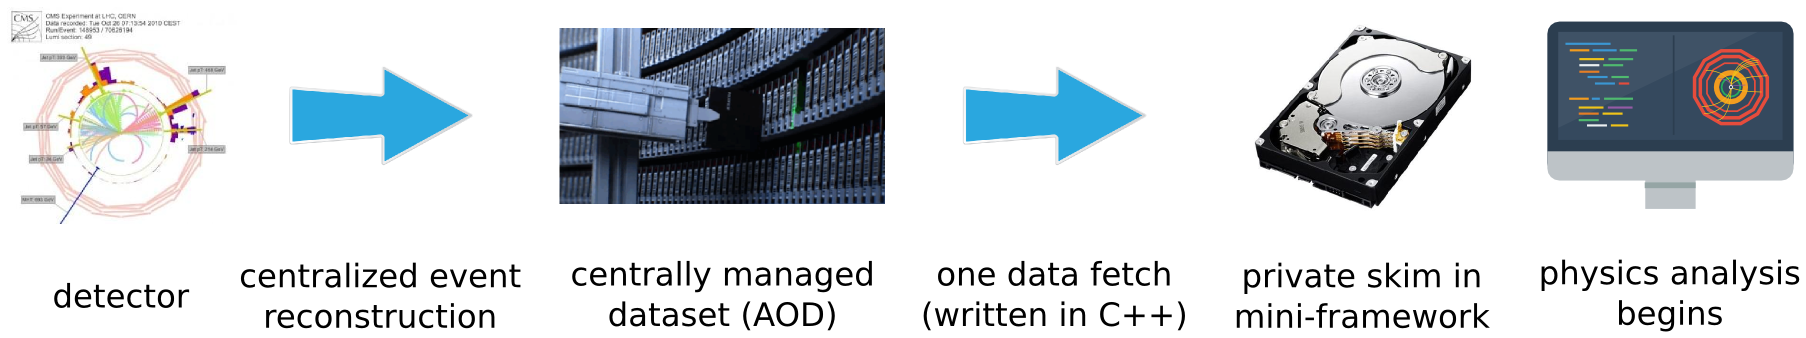
\includegraphics[width=0.8\linewidth]{workflow.png}
\end{center}

\begin{center}
\large \textcolor{darkblue}{with}

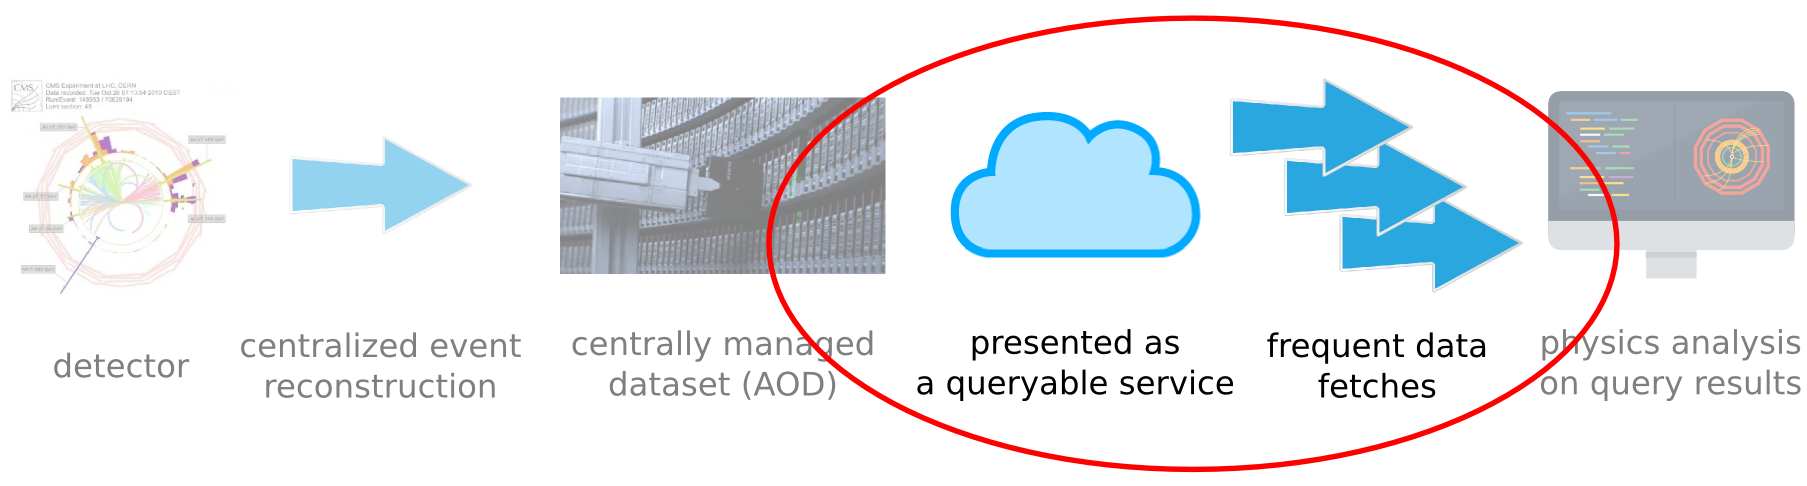
\includegraphics[width=0.8\linewidth]{workflow2.png}
\end{center}

\scriptsize
\vspace{-0.2 cm}
Collaborating with Jin Chang and Igor Mandrichenko on the server.
\end{frame}

\begin{frame}{Why I'm interested in columnar data}
The query language, Femtocode, plays a similar \mbox{role as TTreeFormula:\hspace{-1 cm}}
\begin{itemize}
\item a high-level language for the physicist
\item usually for filling a histogram (so query responses are small)
\item but generally useful for transforming one dataset into another.
\end{itemize}

\vspace{0.3 cm}
However, it's a full-fledged language with assignments and user-defined functions, so that it can encompass a larger part of the data analysis.

\vspace{0.3 cm}
\textcolor{darkgray}{(I've examined SQL, LINQ, and others, and they are not sufficient. I would use a standard if I could. Femtocode BNF has $>$ 50\% overlap with Python BNF.)}
\end{frame}

\begin{frame}{Why I'm interested in columnar data}
The essential feature of Femtocode is that it can compile complex structure-manipulations, which would ordinarily have to be performed in object-oriented code, into a series of vectorized kernels.

\vspace{0.3 cm}
It operates on columns.
\end{frame}

\begin{frame}[fragile]{Data reduction without objects}
\vspace{0.3 cm}
\hspace{-0.25 cm}\textcolor{darkblue}{Example:}
\small
\begin{minted}{python}
  hist = dataset.bin(100, 0, 50, """
      muons.map(m => sqrt(m.px**2 + m.py**2)).max()
  """)
\end{minted}
\normalsize

\vfill
\mbox{\hspace{0.25 cm}\begin{columns}[t]
\column{0.5\linewidth}
\textcolor{darkblue}{compiles to}
\begin{enumerate}
\item Compute $\sqrt{{p_x}^2 + {p_y}^2}$ for all muons, ignoring event boundaries.
\item Find the maximum such value for each event.
\item Bin those events and fill the histogram.
\end{enumerate}

\column{0.5\linewidth}
\normalsize
\textcolor{darkblue}{rather than}
\begin{enumerate}
\item Loop over events:
\begin{enumerate}
\item Loop over muons:
\begin{enumerate}
\item Compute $\sqrt{{p_x}^2 + {p_y}^2}$ for each.
\end{enumerate}
\item Fill a histogram with the maximum.
\end{enumerate}
\end{enumerate}
\end{columns}}
\end{frame}

\begin{frame}{Scope of computability}
\textcolor{darkblue}{Three types of data transformations:}

\vspace{0.2 cm}
\begin{description}\setlength{\itemsep}{0.5 cm}
\item[Flat:] apply $N$-argument function to \\ each element of $N$ aligned \\ arrays, ignoring boundaries.

\vspace{-3\baselineskip}
\hfill 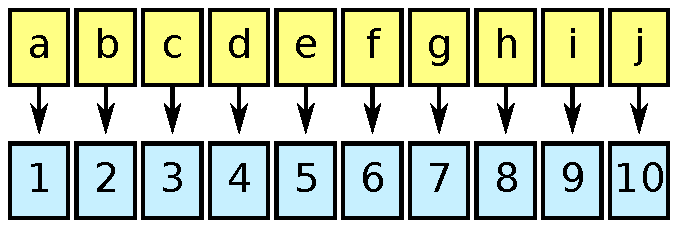
\includegraphics[width=0.37\linewidth]{flat.pdf}

\vspace{0.3 cm}
\item[Explode:] emulate (nested) for-loops by \\ replicating data in one array so \\ that it becomes aligned with \\ another array.

\vspace{-4\baselineskip}
\hfill 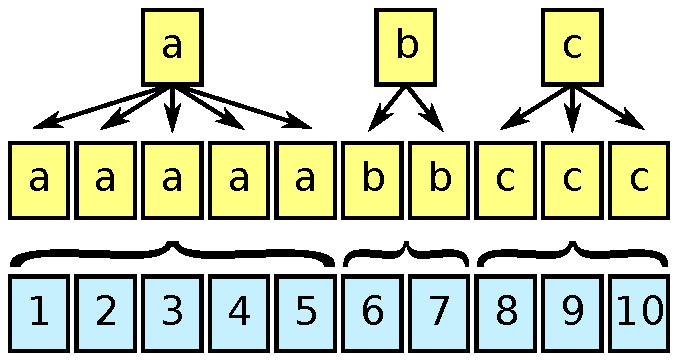
\includegraphics[width=0.37\linewidth]{explode.pdf}

\item[Reduce:] emulate counters, sum, mean, \\ max, etc.\ by combining elements \\ of an array so that it becomes \\ aligned with an outer level of structure.

\vspace{-4\baselineskip}
\hfill 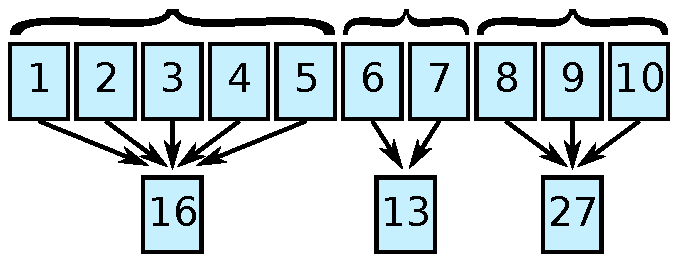
\includegraphics[width=0.37\linewidth]{reduce.pdf}
\end{description}
\end{frame}

\begin{frame}[fragile]{Flat transformations}
\vspace{0.5 cm}
The majority of steps in a typical calculation are flat:

\begin{center}
\begin{minipage}{0.7\linewidth}
\small
\begin{minted}[frame=single]{c++}
double in[ZILLION];
double out[ZILLION];

for (int i = 0;  i < ZILLION;  i++)
  out[i] = flat_operation(in[i]);
\end{minted}
\end{minipage}
\end{center}

\begin{itemize}
\item Compilation with {\tt -O3} vectorizes if possible (depends on {\tt flat\_operation}).
\item Easiest form for CPU to prefetch memory and/or pipeline operations.
\item Also ideal for GPU calculations.
\item There is a standard for functions of this form: Numpy's ufunc is widely used among scientific libraries.
\begin{itemize}
\item Easy way for a user to add functions to the language!
\end{itemize}
\end{itemize}
\end{frame}

\begin{frame}[fragile]{ROOT functions can be ufuncs, too}
\vspace{0.3 cm}
\scriptsize
\begin{minted}{python}
import ctypes, numpy, numba

libMathCore = ctypes.cdll.LoadLibrary("libMathCore.so")
chi2_ctypes = libMathCore._ZN5TMath17ChisquareQuantileEdd # c++filt!
chi2_ctypes.argtypes = (ctypes.c_double, ctypes.c_double)
chi2_ctypes.restype = ctypes.c_double

# compile to pure-C ufunc
@numba.vectorize(["f8(f8, f8)"], nopython=True)
def chi2_ufunc(p, ndf):
    return chi2_ctypes(p, ndf)

p = numpy.random.uniform(0, 1, int(1e6)) # million random numbers
result = chi2_ufunc(p, 100)              # call ufunc on all of them
# 3.22 seconds

import ROOT
result = [ROOT.TMath.ChisquareQuantile(pi, 100) for pi in p]
# 9.32 seconds
\end{minted}

\vspace{0.5 cm}
\textcolor{darkgray}{(Performance comparison is just to show that the ufunc \mbox{computes {\tt ChisquareQuantile}\hspace{-1 cm}}}

\vspace{-0.1 cm}
\textcolor{darkgray}{in C, not in Python. Simpler functions show a more dramatic difference.)}
\end{frame}

\begin{frame}[fragile]{Explode operation}
\vspace{0.3 cm}
Depends critically on the way we represent structure. For the ``recursive counter'' method I described in the last talk,

\vspace{0.3 cm}
\textcolor{darkblue}{Given:} \hfill {\tt [} {\tt [} {\tt a} {\tt b} {\tt c} {\tt ]} {\tt [} {\tt d} {\tt e} {\tt f} {\tt g} {\tt ]} {\tt ]} {\tt [} {\tt [} {\tt h} {\tt ]} {\tt [} {\tt i} {\tt j} {\tt ]} {\tt ]}

\textcolor{darkblue}{Data array:} \hfill {\tt \ } {\tt \ } {\tt a} {\tt b} {\tt c} {\tt \ } {\tt \ } {\tt d} {\tt e} {\tt f} {\tt g} {\tt \ } {\tt \ } {\tt \ } {\tt \ } {\tt h} {\tt \ } {\tt \ } {\tt i} {\tt j} {\tt \ } {\tt \ }

\textcolor{darkblue}{Recursive counter:} \hfill \textcolor{darkorange}{\tt 2} \textcolor{blue}{\tt 3} {\tt \ } {\tt \ } {\tt \ } {\tt \ } \textcolor{blue}{\tt 4} {\tt \ } {\tt \ } {\tt \ } {\tt \ } {\tt \ } {\tt \ } \textcolor{darkorange}{\tt 2} \textcolor{blue}{\tt 1} {\tt \ } {\tt \ } \textcolor{blue}{\tt 2} {\tt \ } {\tt \ } {\tt \ } {\tt \ }

\vspace{0.3 cm}
Calculating arbitrary explosions is solved in two cases:
\begin{itemize}
\item explode scalar to fit a list's counter (35 lines of C)
\item explode list to fit another list's counter (470 lines, recursive).
\end{itemize}

\vspace{-0.3 cm}
\begin{onlyenv}<2>
\begin{center}
\begin{minipage}{0.8\linewidth}
\scriptsize
\vspace{0.3 cm}
\textcolor{darkblue}{Illustration of scalar-to-list:}

\vspace{0.2 cm}
xs $\to$ [1, 2, 3, 4], [], [5, 6, 7] and y $\to$ 100, 200, 300

\vspace{0.2 cm}
Computing
\begin{minted}{scala}
xs.map(x => x + y)
\end{minted}

yields

\vspace{-0.4 cm}
\begin{verbatim}
[101, 102, 103, 104], [], [305, 306, 307]
\end{verbatim}
\end{minipage}
\end{center}
\end{onlyenv}
\begin{onlyenv}<3>
\begin{center}
\begin{minipage}{0.8\linewidth}
\scriptsize
\vspace{0.3 cm}
\textcolor{darkblue}{Illustration of list-to-deeper-list:}

\vspace{0.2 cm}
xss $\to$ [[100, 200], [300, 400], [500, 600]] and ys $\to$ [1, 2, 3, 4]

\vspace{0.2 cm}
Computing
\begin{minted}{scala}
xss.map(xs => xs.map(x => ys.map(y => x + y)))
\end{minted}

yields

\vspace{-0.4 cm}
\begin{verbatim}
[[[101, 102, 103, 104], [201, 202, 203, 204]],
 [[301, 302, 303, 304], [401, 402, 403, 404]],
 [[501, 502, 503, 504], [601, 602, 603, 604]]]
\end{verbatim}
\end{minipage}
\end{center}
\end{onlyenv}
\begin{onlyenv}<4>
\begin{center}
\begin{minipage}{0.8\linewidth}
\scriptsize
\vspace{0.3 cm}
\textcolor{darkblue}{Another illustration of list-to-deeper-list:}

\vspace{0.2 cm}
xss $\to$ [[100, 200], [300, 400], [500, 600]] and ys $\to$ [1, 2, 3, 4]

\vspace{0.2 cm}
Computing
\begin{minted}{scala}
xss.map(xs => ys.map(y => xs.map(x => x + y)))
\end{minted}

yields

\vspace{-0.4 cm}
\begin{verbatim}
[[[101, 201], [102, 202], [103, 203], [104, 204]],
 [[301, 401], [302, 402], [303, 403], [304, 404]],
 [[501, 601], [502, 602], [503, 603], [504, 604]]]
\end{verbatim}
\end{minipage}
\end{center}
\end{onlyenv}
\end{frame}

\begin{frame}{Reduce operations}
Haven't been implemented, but they're pretty straightforward.
\end{frame}

\begin{frame}{Query server}
\vspace{0.4 cm}
Before finishing the language, we want to understand how it will fit into the server.

\vspace{0.2 cm}
\textcolor{darkblue}{Preliminary design:}

\vspace{0.2 cm}
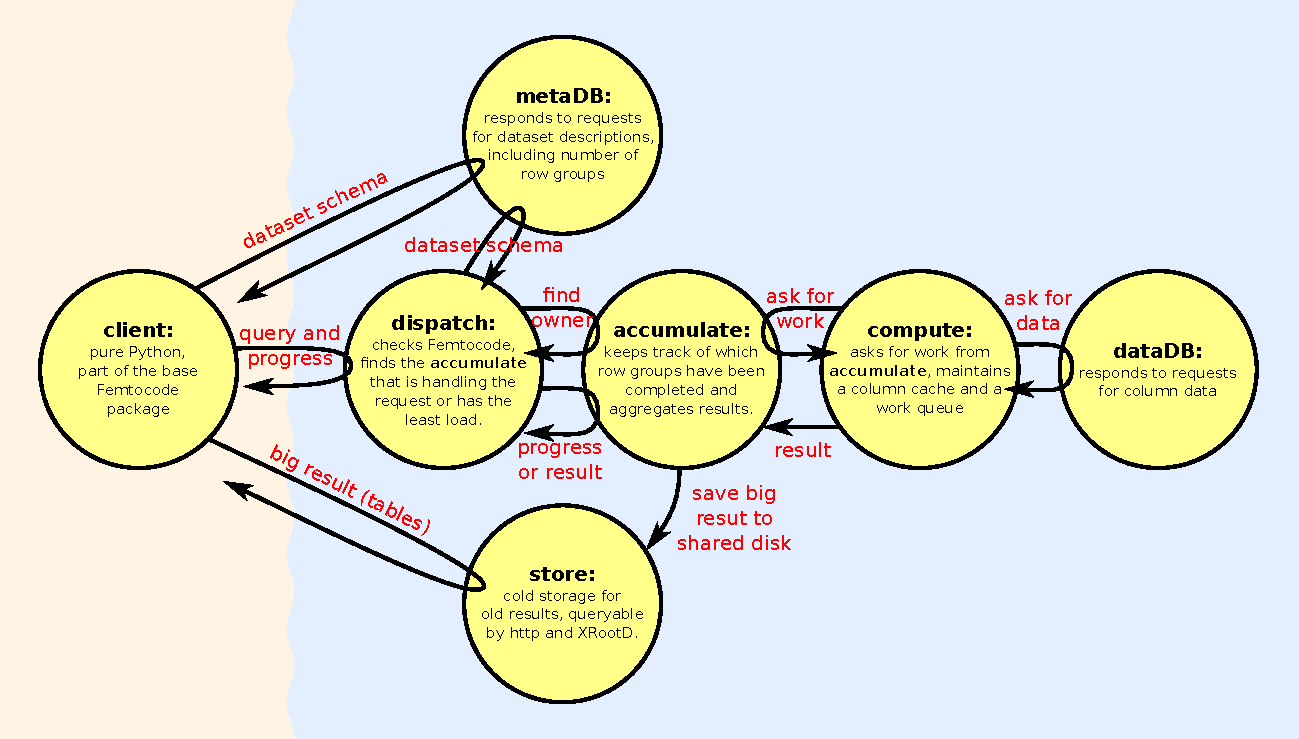
\includegraphics[width=\linewidth]{distributed-system.pdf}
\end{frame}

\begin{frame}{Query server}
If a centralized query server is going to replace private skims, it has to respond to aggregations over whole datasets in seconds.

\vfill
\textcolor{darkblue}{Purpose of early studies:} determine what performance is {\it possible.}
\end{frame}

\begin{frame}{Reading from a CMS MiniAOD file}
\vspace{0.5 cm}
\textcolor{darkblue}{File-reading rates in events/ms per process (kHz per process), with the goal of extracting only $p_T$.}

\mbox{\hspace{-0.5 cm}\begin{tabular}{l c c c c c}
          &         &             &       &{\tt TTree::} & fast \\
particle  &\#/event & \# branches & CMSSW &{\tt Draw()} & reader \\\hline
photon    & 2.9     & 205         & 1.14   &   435       &   769        \\
electron  & 2.5     & 231         & 1.02   &   417       &   833        \\
muon      & 2.7     & 192         & 1.02   &   16.5      &   770        \\
tau       & 6.3     &  88         & 1.55   &   244       &   417        \\
jet       & 16.7    &  95         & 1.15   &   123       &   182        \\
AK8 jet   & 1.8     &  95         & 2.10   &   556       &   1000       \\
\end{tabular}}

\vfill
\small
\begin{itemize}
\item CMSSW loads all branches to reconstruct particles as a C++ objects. Loading all branches just to cut on $p_T$ is wasteful.
\item {\tt TTree::Draw()} is more streamlined, only loads required branches. \textcolor{darkgray}{(Low rate for muons is not understood.)}
\item ``fast reader'' is based on a code snippet Philippe prepared for me, using some of the same techniques as {\tt TTree::Draw()}.
\end{itemize}
\end{frame}

\begin{frame}{Repeated queries on that file}
\vspace{0.5 cm}
We also plan to maintain an in-memory cache of recently used {\it columns,} on the supposition that the column-popularity distribution is steep enough to cause frequent cache-hits among users.

\vspace{0.4 cm}
\textcolor{darkblue}{Rate for simple, \\ flat functions on \\ cached columns is \\ limited only by \\ memory bandwidth.}

\vspace{0.2 cm}
\textcolor{darkblue}{Could reach a peak of \\ 7 GHz on KNL or GPU.}

\vspace{-7\baselineskip}
\vspace{-0.2 cm}
\hfill \mbox{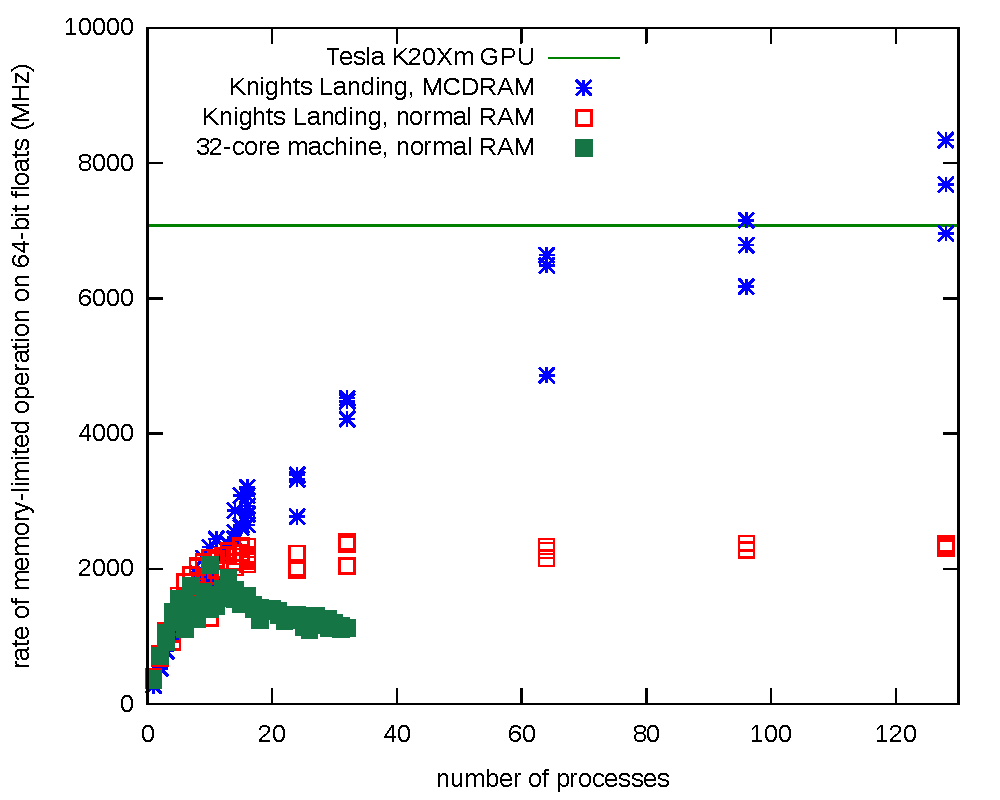
\includegraphics[width=0.7\linewidth]{cleaner.pdf}\hspace{-0.75 cm}}
\end{frame}

\begin{frame}{Conclusions}
\vspace{0.3 cm}
\begin{itemize}\setlength{\itemsep}{0.5 cm}
\item I'm developing Femtocode to translate object semantics into vectorized operations as part of a project to create a fast query server.
\item The ``recursive counter'' representation of nested structure can be exploded and reduced.
\begin{itemize}
\item This representation is identical to ROOT's for depth-1 lists.
\item Any interest in extending to arbitrary split depth?
\end{itemize}
\item Flat functions are
\begin{itemize}
\item quick to compute,
\item extensible using Numpy's ``ufunc'' standard.
\end{itemize}
\item For a cached query server,
\begin{itemize}
\item $\sim$1 MHz column entries is attainable for cache-misses,
\item $\sim$1 GHz column entries is attainable for cache-hits.
\end{itemize}
\end{itemize}
\end{frame}

\end{document}
